% Options for packages loaded elsewhere
\PassOptionsToPackage{unicode}{hyperref}
\PassOptionsToPackage{hyphens}{url}
\PassOptionsToPackage{dvipsnames,svgnames,x11names}{xcolor}
\documentclass[
  spanish,
  11pt,
  a4paper,
]{article}
\usepackage{xcolor}
\usepackage{microtype}
\usepackage[margin=1in]{geometry}
\usepackage{amsmath,amssymb}
\setcounter{secnumdepth}{-\maxdimen} % remove section numbering
\usepackage{iftex}
\ifPDFTeX
  \usepackage[T1]{fontenc}
  \usepackage[utf8]{inputenc}
  \usepackage{textcomp} % provide euro and other symbols
\else % if luatex or xetex
  \usepackage{unicode-math} % this also loads fontspec
  \defaultfontfeatures{Scale=MatchLowercase}
  \defaultfontfeatures[\rmfamily]{Ligatures=TeX,Scale=1}
\setmonofont{Cascadia Mono}
\fi
\usepackage{lmodern}
\ifPDFTeX\else\setmonofont{Cascadia Mono}\fi
\ifPDFTeX\else
  % xetex/luatex font selection
\fi
% Use upquote if available, for straight quotes in verbatim environments
\IfFileExists{upquote.sty}{\usepackage{upquote}}{}
\IfFileExists{microtype.sty}{% use microtype if available
  \usepackage[]{microtype}
  \UseMicrotypeSet[protrusion]{basicmath} % disable protrusion for tt fonts
}{}
\makeatletter
\@ifundefined{KOMAClassName}{% if non-KOMA class
  \IfFileExists{parskip.sty}{%
    \usepackage{parskip}
  }{% else
    \setlength{\parindent}{0pt}
    \setlength{\parskip}{6pt plus 2pt minus 1pt}}
}{% if KOMA class
  \KOMAoptions{parskip=half}}
\makeatother
\usepackage{color}
\usepackage{fancyvrb}
\usepackage{fvextra}
\usepackage[htt]{hyphenat}
\newcommand{\VerbBar}{|}
\newcommand{\VERB}{\Verb[commandchars=\\\{\}]}
\DefineVerbatimEnvironment{Highlighting}{Verbatim}{commandchars=\\\{\},breaklines=true,breakanywhere=true,fontsize=\small}
% Add ',fontsize=\small' for more characters per line
\newenvironment{Shaded}{}{}
\newcommand{\AlertTok}[1]{\textcolor[rgb]{1.00,0.00,0.00}{\textbf{#1}}}
\newcommand{\AnnotationTok}[1]{\textcolor[rgb]{0.38,0.63,0.69}{\textbf{\textit{#1}}}}
\newcommand{\AttributeTok}[1]{\textcolor[rgb]{0.49,0.56,0.16}{#1}}
\newcommand{\BaseNTok}[1]{\textcolor[rgb]{0.25,0.63,0.44}{#1}}
\newcommand{\BuiltInTok}[1]{\textcolor[rgb]{0.00,0.50,0.00}{#1}}
\newcommand{\CharTok}[1]{\textcolor[rgb]{0.25,0.44,0.63}{#1}}
\newcommand{\CommentTok}[1]{\textcolor[rgb]{0.38,0.63,0.69}{\textit{#1}}}
\newcommand{\CommentVarTok}[1]{\textcolor[rgb]{0.38,0.63,0.69}{\textbf{\textit{#1}}}}
\newcommand{\ConstantTok}[1]{\textcolor[rgb]{0.53,0.00,0.00}{#1}}
\newcommand{\ControlFlowTok}[1]{\textcolor[rgb]{0.00,0.44,0.13}{\textbf{#1}}}
\newcommand{\DataTypeTok}[1]{\textcolor[rgb]{0.56,0.13,0.00}{#1}}
\newcommand{\DecValTok}[1]{\textcolor[rgb]{0.25,0.63,0.44}{#1}}
\newcommand{\DocumentationTok}[1]{\textcolor[rgb]{0.73,0.13,0.13}{\textit{#1}}}
\newcommand{\ErrorTok}[1]{\textcolor[rgb]{1.00,0.00,0.00}{\textbf{#1}}}
\newcommand{\ExtensionTok}[1]{#1}
\newcommand{\FloatTok}[1]{\textcolor[rgb]{0.25,0.63,0.44}{#1}}
\newcommand{\FunctionTok}[1]{\textcolor[rgb]{0.02,0.16,0.49}{#1}}
\newcommand{\ImportTok}[1]{\textcolor[rgb]{0.00,0.50,0.00}{\textbf{#1}}}
\newcommand{\InformationTok}[1]{\textcolor[rgb]{0.38,0.63,0.69}{\textbf{\textit{#1}}}}
\newcommand{\KeywordTok}[1]{\textcolor[rgb]{0.00,0.44,0.13}{\textbf{#1}}}
\newcommand{\NormalTok}[1]{#1}
\newcommand{\OperatorTok}[1]{\textcolor[rgb]{0.40,0.40,0.40}{#1}}
\newcommand{\OtherTok}[1]{\textcolor[rgb]{0.00,0.44,0.13}{#1}}
\newcommand{\PreprocessorTok}[1]{\textcolor[rgb]{0.74,0.48,0.00}{#1}}
\newcommand{\RegionMarkerTok}[1]{#1}
\newcommand{\SpecialCharTok}[1]{\textcolor[rgb]{0.25,0.44,0.63}{#1}}
\newcommand{\SpecialStringTok}[1]{\textcolor[rgb]{0.73,0.40,0.53}{#1}}
\newcommand{\StringTok}[1]{\textcolor[rgb]{0.25,0.44,0.63}{#1}}
\newcommand{\VariableTok}[1]{\textcolor[rgb]{0.10,0.09,0.49}{#1}}
\newcommand{\VerbatimStringTok}[1]{\textcolor[rgb]{0.25,0.44,0.63}{#1}}
\newcommand{\WarningTok}[1]{\textcolor[rgb]{0.38,0.63,0.69}{\textbf{\textit{#1}}}}
\usepackage{longtable,booktabs,array}
\newcounter{none} % for unnumbered tables
\usepackage{calc} % for calculating minipage widths
% Correct order of tables after \paragraph or \subparagraph
\usepackage{etoolbox}
\makeatletter
\patchcmd\longtable{\par}{\if@noskipsec\mbox{}\fi\par}{}{}
\makeatother
% Allow footnotes in longtable head/foot
\IfFileExists{footnotehyper.sty}{\usepackage{footnotehyper}}{\usepackage{footnote}}
\makesavenoteenv{longtable}
\usepackage{graphicx}
\makeatletter
\newsavebox\pandoc@box
\newcommand*\pandocbounded[1]{% scales image to fit in text height/width
  \sbox\pandoc@box{#1}%
  \Gscale@div\@tempa{\textheight}{\dimexpr\ht\pandoc@box+\dp\pandoc@box\relax}%
  \Gscale@div\@tempb{\linewidth}{\wd\pandoc@box}%
  \ifdim\@tempb\p@<\@tempa\p@\let\@tempa\@tempb\fi% select the smaller of both
  \ifdim\@tempa\p@<\p@\scalebox{\@tempa}{\usebox\pandoc@box}%
  \else\usebox{\pandoc@box}%
  \fi%
}
% Set default figure placement to htbp
\def\fps@figure{htbp}
\makeatother
\ifLuaTeX
\usepackage[bidi=basic,shorthands=off]{babel}
\else
\usepackage[bidi=default,shorthands=off]{babel}
\fi
\ifLuaTeX
  \usepackage{selnolig} % disable illegal ligatures
\fi
\setlength{\emergencystretch}{8em} % prevent overfull lines
\providecommand{\tightlist}{%
  \setlength{\itemsep}{0pt}\setlength{\parskip}{0pt}}
\usepackage{bookmark}
\IfFileExists{xurl.sty}{\usepackage{xurl}}{} % add URL line breaks if available
\urlstyle{same}
\hypersetup{
  pdftitle={Reducción afín de perfiles para empaquetamientos fraccionales de triángulos en grafos split},
  pdfauthor={AUTHORBLOCK},
  pdflang={es-ES},
  colorlinks=true,
  linkcolor={blue},
  filecolor={Maroon},
  citecolor={Blue},
  urlcolor={blue},
  pdfcreator={LaTeX via pandoc}}

\title{Reducción afín de perfiles para empaquetamientos fraccionales de triángulos en grafos split}
\author{Juan Pablo Traverso Gianini\\
\small Independent researcher, Santiago, Chile\\
\small \href{mailto:jtraverso@gmail.com}{jtraverso@gmail.com}\\
\small ORCID: 0009-0003-6068-4096}
\date{}

% Series layout authority: official GitHub preprint template (article, 11pt, A4, 1in).
% Generated from the language-specific Markdown semantic source.
\AtBeginEnvironment{longtable}{\scriptsize}
\begin{document}
\sloppy
\raggedbottom
\maketitle

\textbf{Paper I de la serie}\\
\textbf{Preprint:} versión 1.3. Este manuscrito y su artefacto formal adjunto forman un único paquete público autocontenido.\\
\textbf{Fecha de publicación:} 22 de agosto de 2026\\
\textbf{Estado:} preprint oficial del autor. El freeze adjunto Paper I Lean v1.2 incluye la evidencia de build registrada y las consultas de axiomas por teorema descritas en la Sección 10. El archivo exacto y el paquete del manuscrito superaron una auditoría adversarial externa independiente. Esta publicación no constituye revisión externa humana por pares ni una determinación especializada de prioridad.

\textbf{Estado del arte previo y la novedad.} La auditoría interna de literatura, complementada por la revisión adversarial externa, no identificó un resultado anterior con la misma cota fraccional finita para grafos split y la misma reducción afín de perfiles. El problema más amplio de particiones en cliques de grafos cordales sigue abierto. Esta es una búsqueda negativa acotada por su corpus, no una demostración de prioridad ni un sustituto de una revisión especializada.

\textbf{MSC 2020:} Primario 05C70; secundarios 05C35, 05C72.

\begin{center}\rule{0.5\linewidth}{0.5pt}\end{center}

\subsection{Resumen}\label{resumen}

Estudiamos empaquetamientos fraccionales de triángulos en grafos split. Una presentación split \(V(G)=K\sqcup I\) permite empaquetar explícitamente los triángulos que intersectan el conjunto independiente. Las capacidades no utilizadas en las aristas de la clique conducen, mediante dualidad finita de programación lineal, a un problema de cobertura de triángulos sobre un único politopo fijo. El vector objetivo de ese problema de cobertura depende afínmente de los tipos de vecindario que aparecen en \(I\).

El mínimo de un objetivo lineal sobre un politopo fijo es cóncavo en el vector objetivo. Esta propiedad de concavidad reduce la tarea de probar una cota inferior uniforme para una mezcla arbitraria de vecindarios del conjunto independiente al análisis de perfiles puros de vecindario. Después de promediar sobre el estabilizador del perfil puro, el problema residual de cobertura se convierte en un programa lineal de tres variables. Resolver ese programa entrega una cota inferior cuadrática uniforme para el valor residual.

Como consecuencia, todo grafo split \(G\) de \(n\) vértices satisface

\[
\boxed{
|E(G)|-2\nu_3^*(G)\le \frac{n^2}{6}+\frac{n}{2},
}
\]

donde \(\nu_3^*(G)\) es el valor máximo de un empaquetamiento fraccional de triángulos. La constante principal \(1/6\) es la que aparece en el Problema \#81 de Erdős sobre particiones en cliques de grafos cordales; el presente resultado se ocupa del problema fraccional finito para la subclase de grafos split. La demostración es finita y analítica. No se usa ningún teorema de transferencia asintótica. La familia complete-split \(K_p\vee\overline{K}_{2p}\) muestra que no es posible un coeficiente aditivo uniforme menor que \(1/6\). Artículos posteriores de la serie obtienen cotas más fuertes para la misma cantidad mediante argumentos independientes y no dependen del presente resultado. Lo que reutilizan es la reducción afín y la tricotomía de tres órbitas resultante.

\textbf{Palabras clave:} grafo split; empaquetamiento fraccional de triángulos; cobertura fraccional de triángulos; programación lineal; reducción afín; simetrización.

\begin{center}\rule{0.5\linewidth}{0.5pt}\end{center}

\subsection{1. Introducción}\label{introducciuxf3n}

Un grafo split es un grafo cuyo conjunto de vértices puede particionarse en una clique y un conjunto independiente. Esta clase es un banco de pruebas natural para problemas de partición en cliques: conserva un núcleo completo rígido y al mismo tiempo permite muchos patrones diferentes de vecindario fuera del núcleo. Erdős, Ordman y Zalcstein {[}1{]} exhibieron ejemplos cordales que requieren asintóticamente \(n^2/6\) cliques y probaron que \((1-c)n^2/4\) cliques bastan para alguna constante absoluta \(c>0\). Para grafos split, Chen, Erdős y Ordman {[}2{]} probaron la cota superior más fuerte \(\frac{3}{16}n^2+O(n)\). El presente artículo estudia, en cambio, el déficit fraccional de empaquetamiento de triángulos \(|E(G)|-2\nu_3^*(G)\), para el cual el resultado siguiente tiene constante principal \(1/6\). Para antecedentes más amplios sobre particiones y coberturas por cliques, véase Cavers {[}5{]}.

El presente artículo aísla un mecanismo fraccional relacionado con el lado split de Erdős Problem \#81 {[}3{]}. En lugar de intentar elegir directamente triángulos arista-disjuntos, construimos primero un empaquetamiento fraccional a partir de triángulos que intersectan el conjunto independiente. La capacidad no utilizada por este primer empaquetamiento permanece en las aristas de la clique, y esas capacidades residuales sostienen un segundo empaquetamiento formado enteramente por triángulos de la clique. La dualidad convierte entonces este problema residual de empaquetamiento en un problema de cobertura fraccional de triángulos sobre la clique.

El punto estructural principal es que el politopo factible de coberturas no depende del perfil de vecindarios del conjunto independiente. Solo cambia el vector objetivo. Como el óptimo de un problema de minimización sobre un politopo fijo es cóncavo en su vector objetivo, un perfil mixto de vecindarios está acotado inferiormente por la correspondiente combinación convexa de valores de perfiles puros y, por tanto, por el menor de esos valores. Esto no identifica un perfil mixto con uno puro; muestra que una cota inferior uniforme puede probarse considerando perfiles puros. El caso puro tiene entonces suficiente simetría para reducirse a tres variables de órbita.

\textbf{Papel dentro del programa más amplio.} Este artículo es autocontenido salvo por el teorema estándar de dualidad fuerte de programación lineal en dimensión finita citado y aplicado en Apéndice B. Su propósito es aislar el mecanismo de reducción afín de perfiles en el contexto split y proporcionar una aplicación fraccional finita. Dentro de la serie sobre Erdős Problem \#81, este mecanismo es el punto de partida: Paper II determina el máximo fraccional exacto del funcional de cobertura sobre grafos cordales; Paper III prueba el teorema de error lineal para particiones en cliques de grafos split; y Paper IV desarrolla una interfaz general de transferencia y redondeo para relajaciones de empaquetamiento dominadas por recursos. Ninguno de esos resultados posteriores se usa aquí.

\textbf{Notación de la serie.} En las comparaciones entre artículos, el déficit fraccional de Paper I se escribe \(\Phi^*(G)=|E(G)|-2\nu_3^*(G)\). Paper II denota la misma cantidad por \(\Phi_\tau(G)=|E(G)|-2\tau_3^*(G)\), mientras que Paper III reserva \(\Phi(G)\), sin estrella, para el déficit integral \(|E(G)|-2\nu_3(G)\). El identificador Lean \texttt{Phi} del artefacto de Paper I se conserva por trazabilidad.

La demostración resultante tiene la forma

\[
\begin{aligned}
\text{empaquetamiento explícito}
&\longrightarrow
\text{politopo residual fijo}\\
&\longrightarrow
\text{reducción afín de perfiles}\\
&\longrightarrow
\text{optimización de tres órbitas}
\end{aligned}
\]

Nuestro teorema principal es finito.

\paragraph{Teorema 1.1}\label{teorema-1.1}

Para todo grafo split \(G\) de \(n\) vértices,

\[
|E(G)|-2\nu_3^*(G)
\le
\frac{n^2}{6}+\frac{n}{2}.
\]

\textbf{Estado de la formalización.} El freeze Paper I Lean v1.2 usa Lean 4 / Mathlib v4.28.0 {[}6,7{]} y registra el Teorema 1.1 como \texttt{paperI\_main\_sharp}. La declaración \texttt{paperI\_main} proporciona una forma compañera más débil con término aditivo \(n\). En estos nombres registrados, \texttt{sharp} se refiere al coeficiente cuadrático \(1/6\), no a la optimalidad del término aditivo. El gate de axiomas cubre el teorema principal, \texttt{PaperI.assembly\_sharp}, \texttt{PaperI.Split.residual\_duality}, la dualidad finita empaquetamiento--cobertura de la Proposición B.1 y las declaraciones de interfaz enumeradas en la Sección 10. Su huella registrada es \texttt{propext}, \texttt{Classical.choice} y \texttt{Quot.sound}, sin axiomas matemáticos propios del proyecto. La Sección 10 presenta el registro del freeze y del archivo.

El ledger de cálculos adjunto registra las identidades exactas, las direcciones de las desigualdades, la estructura de ramas y la contabilidad de pérdidas empleadas en la demostración. El manuscrito mantiene visible, pero compacta, el álgebra rutinaria.

\begin{center}\rule{0.5\linewidth}{0.5pt}\end{center}

\subsection{2. Notación de grafos split}\label{notaciuxf3n-de-grafos-split}

Fijemos una presentación split

\[
V(G)=K\sqcup I,
\]

donde \(K\) es una clique e \(I\) es independiente. Escribimos

\[
p:=|K|.
\]

Para \(v\in I\), sea

\[
d_v:=|N(v)|.
\]

Separamos los vértices independientes en

\[
I_{\ge2}:=\{v\in I:d_v\ge2\},
\qquad
I_1:=\{v\in I:d_v=1\},
\qquad
I_0:=\{v\in I:d_v=0\}.
\]

Definimos

\[
q:=|I_{\ge2}|,
\qquad
b_1:=|I_1|,
\qquad
b_{\ge2}:=\sum_{v\in I_{\ge2}}d_v.
\]

Como no hay aristas dentro de \(I\),

\[
|E(G)|
=
\binom{p}{2}+b_{\ge2}+b_1.
\tag{2.1}
\]

Además,

\[
n=p+q+b_1+|I_0|.
\tag{2.2}
\]

Sea \(\nu_3^*(G)\) el valor máximo de un empaquetamiento fraccional de triángulos: a cada triángulo \(T\) se asigna un peso no negativo \(w(T)\), sujeto a que el peso total de los triángulos que contienen una arista fija sea a lo más uno.

\begin{center}\rule{0.5\linewidth}{0.5pt}\end{center}

\subsection{3. La carga agregada sobre la clique}\label{la-carga-agregada-sobre-la-clique}

Para una arista \(e\in E(K)\) de la clique, definimos

\[
\kappa_e
:=
\sum_{\substack{v\in I_{\ge2}\\ e\subseteq N(v)}}
\frac{1}{d_v-1}.
\tag{3.1}
\]

La normalización se elige de modo que cada vértice independiente activo contribuya en total la mitad de su grado.

\paragraph{Lema 3.1}\label{lema-3.1}

\[
\sum_{e\in E(K)}\kappa_e
=
\frac{b_{\ge2}}2.
\]

\paragraph{Demostración}\label{demostraciuxf3n}

Intercambiamos el orden de sumación:

\[
\begin{aligned}
\sum_{e\in E(K)}\kappa_e
&=
\sum_{v\in I_{\ge2}}
\frac{\binom{d_v}{2}}{d_v-1}\\
&=
\frac12
\sum_{v\in I_{\ge2}}d_v\\
&=
\frac{b_{\ge2}}2.
\end{aligned}
\]

\begin{center}\rule{0.5\linewidth}{0.5pt}\end{center}

\subsection{4. Un empaquetamiento fraccional en dos fases}\label{un-empaquetamiento-fraccional-en-dos-fases}

\begin{figure}
\centering
\pandocbounded{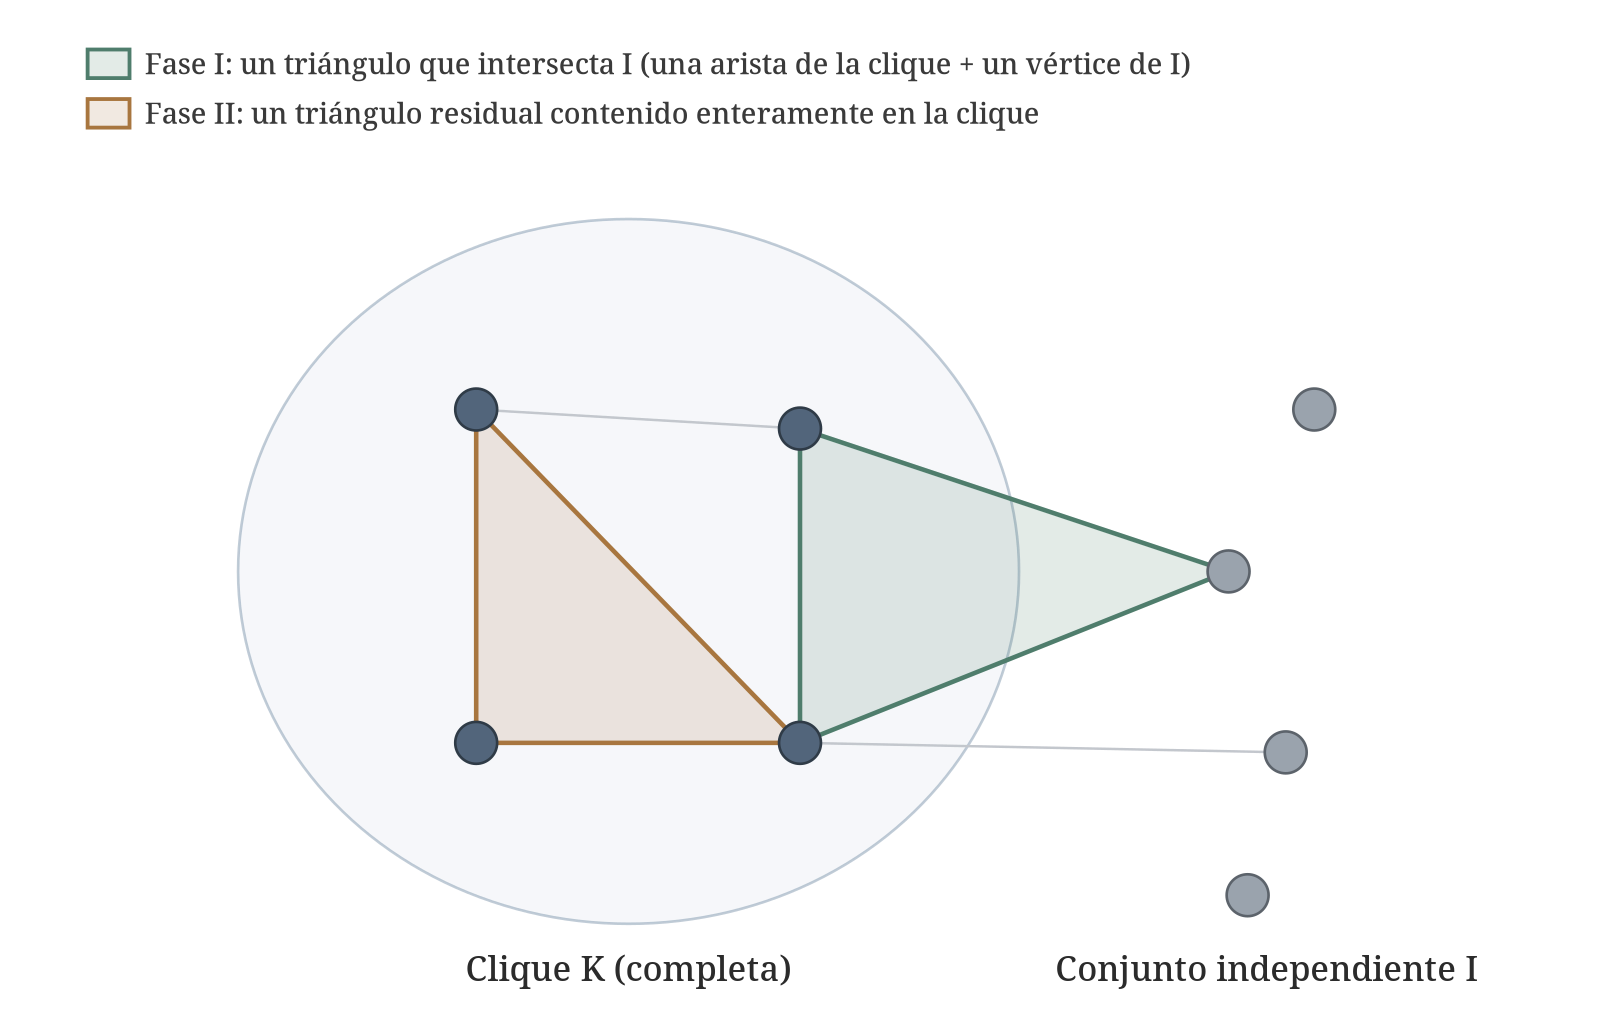
\includegraphics[keepaspectratio,alt={El empaquetamiento fraccional en dos fases.}]{Figures/fig1_two_phase_packing_es.png}}
\caption{El empaquetamiento fraccional en dos fases.}
\end{figure}

\textbf{Figura 1.} El empaquetamiento fraccional en dos fases. La Fase I empaqueta triángulos que intersectan el conjunto independiente (cada uno usa una arista de la clique y un vértice de \(I\)); la capacidad residual que queda en las aristas de la clique sostiene luego la Fase II, un empaquetamiento mediante triángulos contenidos enteramente en la clique.

\subsubsection{4.1 Fase I}\label{fase-i}

Para cada arista \(e\) de la clique, definimos

\[
\lambda_e
:=
\begin{cases}
1,&\kappa_e=0,\\[1mm]
\min\{1,\kappa_e^{-1}\},&\kappa_e>0.
\end{cases}
\]

Para cada triángulo \(vxy\), con \(v\in I_{\ge2}\) y \(x,y\in N(v)\), asignamos

\[
w_1(vxy)
:=
\frac{\lambda_{xy}}{d_v-1}.
\tag{4.1}
\]

La carga sobre una arista \(e\) de la clique es

\[
\lambda_e\kappa_e
=
\min\{\kappa_e,1\}.
\tag{4.2}
\]

Una arista cruzada \(vx\) pertenece a lo más a \(d_v-1\) de estos triángulos, cada uno de peso a lo más \(1/(d_v-1)\). Por tanto, \(w_1\) es factible.

Definimos

\[
H:=\{e:\kappa_e\ge1\},
\qquad
L:=\{e:\kappa_e<1\}.
\]

Todo triángulo de Fase I con peso positivo contiene exactamente una arista de la clique. Por tanto,

\[
|w_1|
=
|H|+\sum_{e\in L}\kappa_e.
\tag{4.3}
\]

\subsubsection{4.2 Fase II}\label{fase-ii}

La capacidad residual sobre una arista de la clique es

\[
r_e:=\max\{1-\kappa_e,0\}.
\tag{4.4}
\]

Sea \(w_2\) un empaquetamiento fraccional óptimo de triángulos de la clique bajo estas capacidades residuales. La dualidad finita empaquetamiento-cobertura usada aquí se registra explícitamente en Apéndice B.

Después de truncar en uno las variables duales de cobertura, sustituimos

\[
y_e:=1-x_e.
\]

Las restricciones de cobertura de triángulos se convierten en

\[
\sum_{e\in E(T)}y_e\le2.
\]

Los coeficientes \(1-\kappa_e\) son no positivos sobre \(H\), de modo que el vector maximizador puede tomarse nulo allí. Una segunda sustitución,

\[
z_e:=1-y_e,
\]

da \(z_e=x_e\) y conduce al politopo dual acotado fijo

\[
\mathcal P_p
:=
\left\{
z\in[0,1]^{E(K)}:
\sum_{e\in E(T)}z_e\ge1
\text{ para todo triángulo }T\subseteq K
\right\}.
\tag{4.5}
\]

Definimos

\[
M(\kappa)
:=
\min_{z\in\mathcal P_p}
\sum_{e\in E(K)}(1-\kappa_e)z_e.
\tag{4.6}
\]

Sean

\[
w_{\mathrm{com}}:=w_1+w_2,
\qquad
V_{\mathrm{com}}:=|w_{\mathrm{com}}|.
\]

Aquí \(M(\kappa)\) es el valor de un problema residual de cobertura, no el valor de un empaquetamiento adicional. Su región factible depende solo del tamaño \(p\) de la clique, mientras toda la información de los vecindarios del conjunto independiente entra mediante los coeficientes objetivo \(1-\kappa_e\).

La contribución de las aristas de \(H\) puede contabilizarse de manera explícita. El Lema 3.1 y (4.3) dan

\[
|w_1|
=
\frac{b_{\ge2}}2+\sum_{e\in H}(1-\kappa_e).
\]

En \(H\), el coeficiente residual \(r_e\) es cero. En (4.6), en cambio, \(1-\kappa_e\le0\); como aumentar \(z_e\) preserva la factibilidad, puede elegirse un minimizador con \(z_e=1\) en toda arista de \(H\). Por tanto, la parte de \(M(\kappa)\) correspondiente a \(H\) es exactamente \(\sum_{e\in H}(1-\kappa_e)\), mientras que su restricción a \(L\) es el valor dual residual \(|w_2|\). De forma equivalente,

\[
|w_2|=M(\kappa)-\sum_{e\in H}(1-\kappa_e).
\]

Al sumar las dos identidades anteriores obtenemos

\[
\boxed{
V_{\mathrm{com}}
=
\frac{b_{\ge2}}2+M(\kappa).
}
\tag{4.7}
\]

El empaquetamiento es factible: sobre una arista de la clique, las cargas de Fase I y residual suman a lo más

\[
\min\{\kappa_e,1\}
+
\max\{1-\kappa_e,0\}
=
1.
\]

En consecuencia,

\[
V_{\mathrm{com}}\le\nu_3^*(G).
\tag{4.8}
\]

Al combinar (2.1) y (4.7) obtenemos

\[
\boxed{
|E(G)|-2V_{\mathrm{com}}
=
\binom{p}{2}-2M(\kappa)+b_1.
}
\tag{4.9}
\]

Esta cancelación es el puente entre la construcción de empaquetamiento y el problema de perfiles.

\begin{center}\rule{0.5\linewidth}{0.5pt}\end{center}

\subsection{5. Reducción afín a un vecindario puro}\label{reducciuxf3n-afuxedn-a-un-vecindario-puro}

Para todo conjunto \(S\subseteq K\) con \(|S|\ge2\), definimos

\[
a_e^S
:=
\frac{\mathbf1_{\{e\subseteq S\}}}{|S|-1}.
\tag{5.1}
\]

Sea \(n_S\) el número de vértices \(v\in I_{\ge2}\) con \(N(v)=S\). Entonces

\[
\kappa=\sum_Sn_Sa^S.
\tag{5.2}
\]

Supongamos primero que \(q>0\) y definamos

\[
\lambda_S:=\frac{n_S}{q},
\qquad
\kappa^S:=qa^S.
\]

Entonces

\[
\kappa=\sum_S\lambda_S\kappa^S,
\qquad
\lambda_S\ge0,
\qquad
\sum_S\lambda_S=1.
\tag{5.3}
\]

La reducción se sigue de un hecho elemental de concavidad.

\paragraph{Lema 5.1}\label{lema-5.1}

Sea \(P\) no vacío y definamos la función valor

\[
m(c):=\min_{x\in P}\langle c,x\rangle.
\]

Si \(c=\sum_i\lambda_ic^{(i)}\) es una combinación convexa, entonces

\[
m(c)
\ge
\sum_i\lambda_i m(c^{(i)})
\ge
\min_i m(c^{(i)}).
\]

\paragraph{Demostración}\label{demostraciuxf3n-1}

Para todo \(x\in P\),

\[
\langle c,x\rangle
=
\sum_i\lambda_i\langle c^{(i)},x\rangle
\ge
\sum_i\lambda_i m(c^{(i)}).
\]

Tomamos el mínimo sobre \(x\in P\).

El valor residual de Sección 4.2 satisface \(M(\kappa)=m(1-\kappa)\) cuando el politopo genérico es \(P=\mathcal P_p\); las letras diferentes distinguen el lema genérico de concavidad de la notación residual específica del manuscrito.

Aplicamos el lema a los vectores objetivo \(1-\kappa^S\) sobre el politopo fijo \(\mathcal P_p\). La conclusión es una reducción de cota inferior: un perfil mixto no tiene por qué coincidir con ningún perfil puro, pero su valor residual es al menos el promedio correspondiente de los valores de perfiles puros. Obtenemos

\[
\boxed{
M(\kappa)
\ge
\sum_S\lambda_SM(\kappa^S)
\ge
\min_SM(\kappa^S).
}
\tag{5.4}
\]

Resta controlar un perfil puro.

\begin{center}\rule{0.5\linewidth}{0.5pt}\end{center}

\paragraph{Observación (concavidad sobre un politopo fijo)}\label{observaciuxf3n-concavidad-sobre-un-politopo-fijo}

La reducción que acabamos de usar es un caso de un hecho puramente convexo-analítico, que formulamos aquí de manera abstracta. Fijemos un politopo factible que no dependa del perfil y una función objetivo que dependa afínmente de la masa del perfil \(\mu=(\mu_S)\). Como el valor óptimo de un programa lineal sobre un politopo fijo es cóncavo respecto de su vector objetivo, el valor en un perfil mixto domina la combinación convexa correspondiente de los valores de los perfiles puros y, por tanto, también su mínimo:
\[
M_b(\kappa_\mu)\ \ge\ \sum_S \tfrac{\mu_S}{q}\,M_b(\kappa^{S,q})\ \ge\ \min_S M_b(\kappa^{S,q}).
\]
Esto se registra en el desarrollo formal como \texttt{lpVal\_concave} y \texttt{lpVal\_ge\_min}. Una estimación complementaria, \texttt{lpVal\_lipschitz}, acota la variación del valor fraccional cuando se perturban el baseline o la distribución de perfiles. Está pensada para variantes robustas y casi split. Ambas se formulan para un politopo factible fijo con una función objetivo que varía afínmente; ninguna requiere simetría, que solo interviene después, sobre un único perfil puro, en la Sección 6.

\subsection{6. El programa de órbitas del perfil puro}\label{el-programa-de-uxf3rbitas-del-perfil-puro}

\begin{figure}
\centering
\pandocbounded{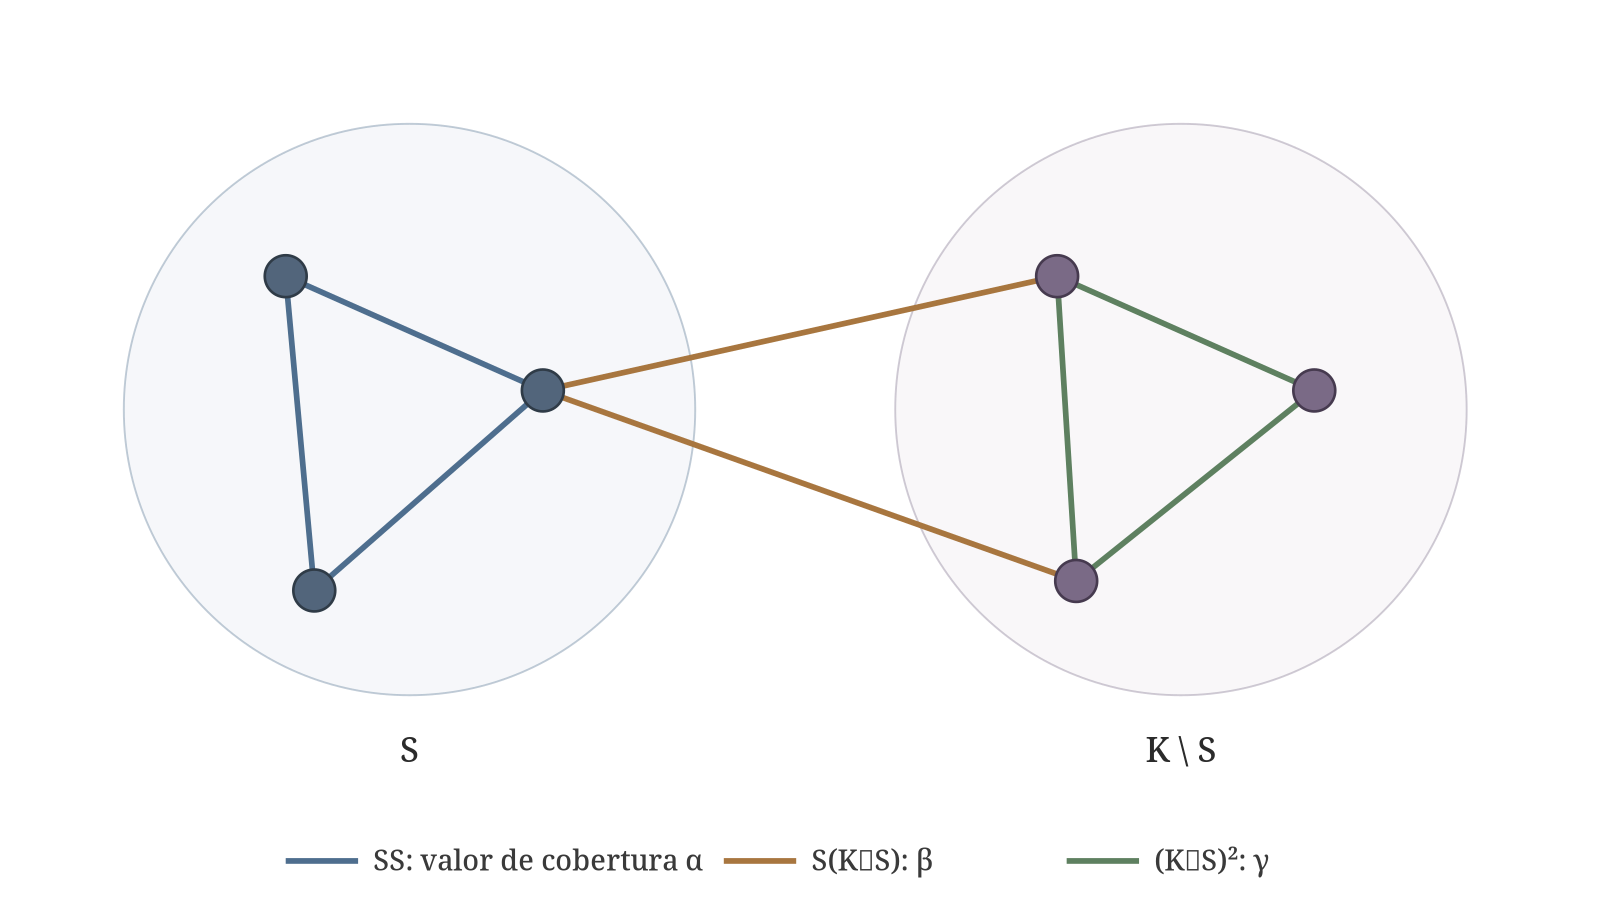
\includegraphics[keepaspectratio,alt={Las tres órbitas de aristas de un perfil puro.}]{Figures/fig2_three_orbits_es.png}}
\caption{Las tres órbitas de aristas de un perfil puro.}
\end{figure}

\textbf{Figura 2.} Para un perfil puro \(S\subseteq K\), las aristas de la clique se dividen en tres órbitas --- \(SS\), \(S(K\setminus S)\) y \((K\setminus S)(K\setminus S)\) --- sobre las cuales la cobertura promediada es constante, con valores \(\alpha,\beta,\gamma\), respectivamente.

Fijemos \(S\subseteq K\) y escribamos

\[
s:=|S|,
\qquad
o:=p-s.
\]

Para el perfil puro,

\[
\kappa_e^S
=
\begin{cases}
q/(s-1),&e\subseteq S,\\
0,&\text{en otro caso}.
\end{cases}
\tag{6.1}
\]

Promediamos una cobertura óptima sobre el estabilizador de \(S\). Tanto el politopo de coberturas como el objetivo del perfil puro son invariantes bajo este grupo. Por tanto, el promedio preserva la factibilidad y el valor objetivo. La cobertura promediada es constante sobre las tres órbitas de aristas:

\[
SS,\qquad
S(K\setminus S),\qquad
(K\setminus S)(K\setminus S).
\]

Llamemos a los valores correspondientes

\[
\alpha,\qquad\beta,\qquad\gamma.
\]

El objetivo es

\[
A\alpha+B\beta+C\gamma,
\tag{6.2}
\]

donde

\[
A:=\frac{s(s-1-q)}2,
\qquad
B:=so,
\qquad
C:=\frac{o(o-1)}2.
\tag{6.3}
\]

Los tipos de triángulos existentes imponen

\[
3\alpha\ge1,
\qquad
\alpha+2\beta\ge1,
\qquad
2\beta+\gamma\ge1,
\qquad
3\gamma\ge1,
\tag{6.4}
\]

omitiéndose toda restricción cuyo tipo de triángulo no exista.

La región factible es ahora un politopo tridimensional. Sus puntos extremos relevantes proporcionan las coberturas uniforme, separada y de conjunto caliente; cuando algunos tipos de triángulo no existen, los regímenes de frontera correspondientes deben tratarse por separado. Resolver este programa de tres variables da

\[
M(\kappa^S)
=
\begin{cases}
\min\{U,D\},&o\le2,\\[1mm]
\min\{U,D,H\},&o\ge3,
\end{cases}
\tag{6.5}
\]

donde

\[
U:=\frac{A+B+C}{3},
\qquad
D:=A+C,
\qquad
H:=A+\frac{B+C}{3}.
\tag{6.6}
\]

Los tres valores corresponden a la cobertura uniforme, la cobertura separada y la cobertura de conjunto caliente.

\textbf{Tabla 1. El programa de cobertura de tres órbitas.} Para un perfil puro \(S\subseteq K\), con \(s=|S|\) y \(o=p-s\), el objetivo residual es \(A\alpha+B\beta+C\gamma\) sobre las órbitas de aristas \(SS\), \(S(K\setminus S)\), \((K\setminus S)(K\setminus S)\), y su mínimo se alcanza en una de tres coberturas nombradas.

{\def\LTcaptype{none} % do not increment counter
\begin{longtable}[]{@{}lll@{}}
\toprule\noalign{}
Cobertura & Valor & Valores de órbita \((\alpha,\beta,\gamma)\) \\
\midrule\noalign{}
\endhead
\bottomrule\noalign{}
\endlastfoot
Uniforme \(U\) & \((A+B+C)/3\) & \((\tfrac13,\tfrac13,\tfrac13)\) \\
Separada \(D\) & \(A+C\) & \((1,0,1)\) \\
Conjunto caliente \(H\) & \(A+(B+C)/3\) & \((1,\tfrac13,\tfrac13)\) \\
\end{longtable}
}

con \(A=\tfrac{s(s-1-q)}2\), \(B=so\), \(C=\tfrac{o(o-1)}2\); y \(M(\kappa^S)=\min\{U,D\}\) para \(o\le2\), \(\min\{U,D,H\}\) para \(o\ge3\) (Apéndice A).

\begin{center}\rule{0.5\linewidth}{0.5pt}\end{center}

\subsection{7. Una cota inferior uniforme para la cobertura residual}\label{una-cota-inferior-uniforme-para-la-cobertura-residual}

Definimos

\[
R(p,q)
:=
\frac{2p^2-2pq-q^2}{12}.
\tag{7.1}
\]

Comparamos cada candidato de (6.5) con \(R(p,q)\).

Para el candidato uniforme, usando \(o=p-s\),

\[
12(U-R)
=
q(2o+q)-2p.
\tag{7.2}
\]

Como \(q,o\ge0\),

\[
U-R\ge-\frac p6.
\tag{7.3}
\]

Para el candidato separado,

\[
12(D-R)
=
12o^2-6o(2p-q)+(2p-q)^2-6p.
\tag{7.4}
\]

La parte cuadrática es no negativa porque

\[
12u^2-6uv+v^2
=
12\left(u-\frac v4\right)^2+\frac{v^2}{4}.
\]

Por tanto,

\[
D-R\ge-\frac p2.
\tag{7.5}
\]

Para el candidato de conjunto caliente,

\[
12(H-R)
=
(2s-q)^2+2q(p-s)-2p-4s.
\tag{7.6}
\]

Los dos primeros términos son no negativos, y \(s\le p\), de modo que

\[
H-R\ge-\frac p2.
\tag{7.7}
\]

En consecuencia,

\[
M(\kappa^S)
\ge
R(p,q)-\frac p2
\]

para todo perfil puro. Por (5.4),

\[
\boxed{
M(\kappa)
\ge
R(p,q)-\frac p2.
}
\tag{7.8}
\]

Cuando \(q=0\), la misma estimación se sigue directamente. Si \(p\le2\), entonces \(M(0)=0\). Si \(p\ge3\), la cobertura constante \(z_e=1/3\) es factible. Para ver que es óptima, sumamos las restricciones de cobertura sobre todos los triángulos de la clique: cada arista de la clique aparece en exactamente \(p-2\) de estos triángulos, lo que da la cota inferior coincidente. Por tanto,

\[
M(0)=\frac{p(p-1)}6.
\]

\begin{center}\rule{0.5\linewidth}{0.5pt}\end{center}

\paragraph{Observación (dónde la estimación es ajustada)}\label{observaciuxf3n-duxf3nde-la-estimaciuxf3n-es-ajustada}

Las tres comparaciones anteriores están lejos de ser ajustadas salvo en una configuración. Escribiendo \(o=p-s\), la holgura \(M(\kappa^S)-\big(R(p,q)-p/2\big)\) es al menos \(9/4\) cuando \(s\ge3\) y \(o\ge3\), y al menos \(1/4\) en cada uno de los regímenes \(s=2\) con \(o\ge1\), \(o=1\) y \(o=2\). La igualdad ocurre únicamente cuando \(o=0\) y \(q=2p\): el perfil puro cuyo vecindario es toda la clique en un grafo con \(|I|=2|K|\), que es precisamente el extremizador complete-split \(K_p\vee\overline K_{2p}\) evaluado en la Sección 9 e identificado por Paper II como la familia terminal del problema extremal fraccional. Por tanto, el punto \((p,q,s)=(2,4,2)\) de la frontera \(s=2\) pertenece a la familia de igualdad; fuera de \(o=0\), esa frontera tiene holgura al menos \(1/4\). El Apéndice A trata los regímenes de borde por completo porque el mínimo del programa de órbitas cambia realmente de forma allí.

\subsection{8. Demostración del teorema principal}\label{demostraciuxf3n-del-teorema-principal}

Partimos de (4.9):

\[
|E(G)|-2V_{\mathrm{com}}
=
\binom p2-2M(\kappa)+b_1.
\]

Insertamos (7.8):

\[
|E(G)|-2V_{\mathrm{com}}
\le
\binom p2-2R(p,q)+p+b_1.
\tag{8.1}
\]

Una simplificación directa da

\[
\binom p2-2R(p,q)+p
=
\frac{(p+q)^2}{6}+\frac p2.
\tag{8.2}
\]

Por tanto,

\[
|E(G)|-2V_{\mathrm{com}}
\le
\frac{(p+q)^2}{6}+\frac p2+b_1.
\tag{8.3}
\]

Escribamos \(n=p+q+b_1+|I_0|\) a partir de (2.2), donde \(I_0\) es el conjunto de vértices independientes aislados. En vez de acotar por separado los términos cuadrático y lineal de (8.3), restamos (8.3) del objetivo cuyo coeficiente cuadrático es afilado:

\[
\frac{n^2}{6}+\frac n2-\Big[\frac{(p+q)^2}{6}+\frac p2+b_1\Big]
=
\frac{b_1^2+|I_0|^2+2b_1|I_0|+2(b_1+|I_0|)(p+q)+3|I_0|+3q-3b_1}{6}.
\]

Todos los términos del lado derecho son no negativos salvo \(-3b_1\). Si \(b_1=0\), la desigualdad es inmediata. Si \(b_1\ge1\), entonces \(p\ge1\), pues un vértice independiente de grado uno tiene su vecino en \(K\); al agrupar \(2b_1(p+q)-3b_1=b_1(2p+2q-3)\), se ve que esta cantidad es no negativa siempre que \(p+q\ge2\). El régimen residual es \(p=1,\ q=0\), donde la diferencia se reduce a

\[
\frac{b_1(b_1-1)+|I_0|^2+2b_1|I_0|+5|I_0|}{6}\ge0,
\]

con igualdad exactamente cuando \(b_1=1\) y \(|I_0|=0\). Por consiguiente,

\[
|E(G)|-2V_{\mathrm{com}}
\le
\frac{n^2}{6}+\frac n2.
\tag{8.4}
\]

Finalmente, \(V_{\mathrm{com}}\le\nu_3^*(G)\). Así,

\[
|E(G)|-2\nu_3^*(G)
\le
|E(G)|-2V_{\mathrm{com}}
\le
\frac{n^2}{6}+\frac n2.
\]

Esto prueba el Teorema 1.1.

\begin{center}\rule{0.5\linewidth}{0.5pt}\end{center}

\subsection{9. Discusión}\label{discusiuxf3n}

Tres ideas elementales impulsan la demostración. Primero separamos el empaquetamiento en una parte sostenida por triángulos que intersectan el conjunto independiente y una parte residual sostenida enteramente por la clique. Luego formulamos el problema residual sobre un único politopo fijo de coberturas. La simetría se usa solo después de reducir el problema de cota inferior a perfiles puros.

La característica de politopo fijo es el punto estructural central. La concavidad se aplica porque la región factible no cambia cuando cambia el perfil de vecindarios; solo cambia el vector objetivo. Si las propias restricciones dependieran del perfil, la reducción de Sección 5 ya no se seguiría del mismo argumento. El promedio sobre órbitas es un paso separado: usa la simetría de un perfil puro y no es necesario para la reducción afín en sí.

Las cantidades intermedias \(p\), \(q\) y \(\kappa\) dependen de la presentación split elegida. La estimación final no. Una vez ensamblados los términos, la conclusión se expresa únicamente en función de \(n=|V(G)|\).

El término aditivo \(n/2\) del Teorema 1.1 no está optimizado. Para la familia complete-split \(K_p\vee\overline{K}_{2p}\), con \(p\ge2\) y \(n=3p\), todo triángulo usa al menos una arista de la clique, de modo que \(\nu_3^*(G)\le\binom p2\), mientras que la construcción de Fase I alcanza la igualdad. En consecuencia, el lado izquierdo del Teorema 1.1 es \(n^2/6+n/6\) sobre esta familia, por lo que el término aditivo óptimo se encuentra entre \(n/6\) y el \(n/2\) demostrado aquí. Determinarlo exactamente queda fuera del alcance del presente argumento.

El artículo se limita deliberadamente a la desigualdad fraccional finita. Todo paso hacia empaquetamientos integrales de triángulos, particiones en cliques, consecuencias asintóticas o clases de grafos más amplias requiere resultados adicionales y pertenece a una etapa separada.

El componente reutilizable es la reducción afín sobre un politopo fijo, independiente de la cota finita particular probada aquí.

Paper III de la serie reutiliza posteriormente el mismo cálculo de tres órbitas para perfiles puros en un contexto integral. Con su notación \(d=s\) y \(p-d=o\), las tres ramas de su valor de perfil común \(F(p,q,d)\) son \(qd/2+U\), \(qd/2+D\) y \(qd/2+H\), donde \(qd/2\) es la contribución de Fase I del perfil puro del presente artículo; su término \(C_\alpha p^2\), para \(\alpha=q/p\), es el valor de comparación \(R(p,q)\) de la Sección 7. Esta es solo una referencia prospectiva: no se usa aquí ningún resultado de Paper III.

\begin{center}\rule{0.5\linewidth}{0.5pt}\end{center}

\subsection{10. Reproducibilidad y registro de la demostración}\label{reproducibilidad-y-registro-de-la-demostraciuxf3n}

La demostración es analítica. Durante el desarrollo se usaron experimentos computacionales para buscar contraejemplos y detectar errores de transcripción, pero ningún cálculo es una premisa lógica del teorema. Por esa razón, el material de regresión computacional se mantiene fuera del artículo, en lugar de incluirse como un segundo apéndice.

El ledger de cálculos adjunto registra:

\begin{itemize}
\tightlist
\item
  cada identidad exacta;
\item
  cada dirección de desigualdad;
\item
  la contabilidad completa de pérdidas;
\item
  la rama \(q=0\);
\item
  los regímenes de órbitas;
\item
  la conversión final a \(n\).
\end{itemize}

El autor reporta una auditoría adversarial interna asistida por IA del enunciado del teorema, la cota cuantitativa y el ensamblaje de la demostración. Este es un registro de validación, no una afirmación de revisión externa por pares.

\subsubsection{Estado de formalización en Lean}\label{estado-de-formalizaciuxf3n-en-lean}

El snapshot en \texttt{PAPER\_I/05\_formalization/lean\_v1.2\_freeze} contiene las fuentes Lean y un build registrado exitoso de 8.034 jobs con Lean 4 / Mathlib v4.28.0 {[}6,7{]}. Contiene \texttt{paperI\_main\_sharp}, cuyo enunciado es \texttt{Phi\ ≤\ n\^{}2/6\ +\ n/2}, junto con la declaración compañera más débil \texttt{paperI\_main} y los resultados de interfaz enumerados más abajo. Su gate de axiomas también consulta \texttt{PaperI.assembly\_sharp} y \texttt{PaperI.Split.residual\_duality}. El Apéndice C registra la declaración principal. Posteriormente, el archivo exacto se reprodujo en un clean room externo con el mismo resultado de 8.034 jobs y la misma huella axiomática por teorema.

El informe de axiomas congelado registra únicamente los axiomas fundacionales estándar de Lean, \texttt{propext}, \texttt{Classical.choice} y \texttt{Quot.sound}, para el teorema principal y las declaraciones enumeradas; no registra ningún axioma matemático propio del proyecto. Se trata de fundamentos lógicos usados en todo Mathlib, no de supuestos matemáticos adicionales del artículo.

El artefacto de release también registra la dualidad finito-dimensional empaquetamiento-cobertura usada en Proposición B.1. En Lean aparece como \texttt{residual\_duality}, una aplicación del teorema general \texttt{covering\_packing\_duality}. El artefacto registra este último teorema como derivado de un lema de Farkas finito y de la infraestructura de conos cerrados de Mathlib, en lugar de postularlo como un axioma externo. Schrijver {[}4, Capítulo 7{]} sigue siendo la referencia clásica para la demostración escrita.

El archivo de fuentes congelado es \texttt{PAPER\_I\_lean\_v1.2\_freeze.zip}, con SHA-256 \texttt{0181506408644fc1f8872d711de5a98a500f4052aa295bcd6f8c82776694fd3a}. Se almacena bajo \texttt{PAPER\_I/05\_formalization/lean\_v1.2\_freeze} y excluye los caches del proyecto y los objetos compilados. El target del build congelado incluye varios módulos \texttt{Contrib} destinados a un posible upstream; esa vía de contribución es un subproducto y no forma parte de los supuestos matemáticos de confianza del artículo. El informe de axiomas anterior controla la afirmación sobre dependencias lógicas. La reproducción externa en clean room corresponde exactamente a estos bytes del archivo; la revisión del manuscrito no modifica el artefacto formal.

\begin{center}\rule{0.5\linewidth}{0.5pt}\end{center}

\subsection{Apéndice A. El programa de tres órbitas y sus casos de frontera}\label{apuxe9ndice-a.-el-programa-de-tres-uxf3rbitas-y-sus-casos-de-frontera}

Este apéndice proporciona los detalles detrás de (6.5). Se incluye porque los casos en que uno de los cuatro tipos de triángulo no existe pueden quedar fácilmente ocultos en un cálculo comprimido de órbitas.

Para un perfil puro \(S\subseteq K\), escribimos

\[
s:=|S|,
\qquad
o:=p-s,
\]

y sean \(\alpha,\beta,\gamma\) los valores de cobertura sobre las órbitas de aristas

\[
SS,\qquad S(K\setminus S),\qquad (K\setminus S)(K\setminus S).
\]

El objetivo es

\[
A\alpha+B\beta+C\gamma,
\]

donde

\[
A=\frac{s(s-1-q)}2,
\qquad
B=so,
\qquad
C=\frac{o(o-1)}2.
\]

Solo se imponen las restricciones correspondientes a tipos de triángulo existentes.

\subsubsection{\texorpdfstring{A.1 El caso interior \(s\ge3\) y \(o\ge3\)}{A.1 El caso interior s\textbackslash ge3 y o\textbackslash ge3}}\label{a.1-el-caso-interior-sge3-y-oge3}

Están presentes las cuatro restricciones:

\[
3\alpha\ge1,
\qquad
\alpha+2\beta\ge1,
\qquad
2\beta+\gamma\ge1,
\qquad
3\gamma\ge1.
\]

Si \(A<0\), disminuir el objetivo favorece el mayor valor factible de \(\alpha\), de modo que un óptimo tiene \(\alpha=1\). La frontera inferior restante une

\[
(\beta,\gamma)=(0,1)
\]

y

\[
(\beta,\gamma)=\left(\frac13,\frac13\right).
\]

Como el objetivo es lineal sobre ese segmento, su mínimo se alcanza en un extremo. Los valores de esos dos extremos son

\[
D=A+C
\]

y

\[
H=A+\frac{B+C}{3}.
\]

Si \(A\ge0\), entonces, para \(\beta\) fijo, los menores valores factibles de \(\alpha\) y \(\gamma\) son

\[
\alpha=\gamma=\max\left\{\frac13,1-2\beta\right\}.
\]

Para \(0\le\beta\le1/3\), el objetivo es lineal entre el punto separado y el punto uniforme, con valores \(D\) y

\[
U=\frac{A+B+C}{3}.
\]

Para \(\beta\ge1/3\), el objetivo es

\[
U+B\left(\beta-\frac13\right)\ge U,
\]

porque \(B\ge0\). Por tanto, el mínimo es uno de \(U,D,H\).

\subsubsection{\texorpdfstring{A.2 El caso \(s=2\)}{A.2 El caso s=2}}\label{a.2-el-caso-s2}

El tipo de triángulo \(SSS\) no existe, por lo que se omite la restricción \(3\alpha\ge1\).

Si \(A<0\), el mismo argumento de monotonicidad da \(\alpha=1\), y el análisis de extremos anterior sigue siendo válido.

Si \(A\ge0\) y \(o\ge3\), la restricción ausente introduce un extremo adicional de frontera en \(\beta=1/2\). Su valor objetivo excede el valor uniforme en

\[
\frac{B-2A}{6}.
\]

Para \(s=2\),

\[
B-2A
=
2o-2(1-q)
=
2(o+q-1)\ge0
\]

siempre que este extremo sea pertinente. Por tanto, no mejora \(U\). Los casos \(o=0,1,2\), en los que faltan algunos tipos de triángulos y sus restricciones, se tratan por separado en A.3; la fórmula anterior para el exceso no se usa allí.

\subsubsection{\texorpdfstring{A.3 Los casos \(o=0,1,2\)}{A.3 Los casos o=0,1,2}}\label{a.3-los-casos-o012}

Cuando \(o=0\), tenemos \(B=C=0\). Si \(s\ge3\), la única restricción de triángulo es \(3\alpha\ge1\), de modo que

\[
\min_{\alpha\in[1/3,1]}A\alpha
=
\min\left\{\frac A3,A\right\}
=
\min\{U,D\}.
\]

Si \(s=2\), entonces \(p=2\) y no hay restricciones provenientes de triángulos de la clique. Como el caso de perfil puro tiene \(q>0\), tenemos \(A=1-q\le0\), y el mínimo sobre \(0\le\alpha\le1\) es \(A=D\). Así, la fórmula \(\min\{U,D\}\) sigue siendo válida.

Cuando \(o=1\), no hay aristas \((K\setminus S)^2\) ni un tipo de triángulo contenido enteramente en \(K\setminus S\). La región factible reducida es un intervalo, y sus extremos dan \(U\) o \(D\).

Cuando \(o=2\), no existe el tipo de triángulo contenido enteramente en \(K\setminus S\). Un posible extremo adicional tiene

\[
(\beta,\gamma)=\left(\frac12,0\right)
\]

y valor objetivo

\[
A+\frac B2.
\]

Como \(o=2\),

\[
\frac B2=s
\qquad\text{y}\qquad
C=1,
\]

por lo que

\[
A+\frac B2\ge A+C=D.
\]

Así, este extremo está dominado por \(D\).

En consecuencia,

\[
M(\kappa^S)
=
\begin{cases}
\min\{U,D\},&o\le2,\\[1mm]
\min\{U,D,H\},&o\ge3.
\end{cases}
\]

No se usa ninguna órbita inexistente ni ninguna restricción de triángulo inexistente en los regímenes de frontera.

\begin{center}\rule{0.5\linewidth}{0.5pt}\end{center}

\subsection{Apéndice B. Dualidad finita empaquetamiento-cobertura}\label{apuxe9ndice-b.-dualidad-finita-empaquetamiento-cobertura}

Para completar la exposición, registramos el par dual finito especializado de empaquetamiento-cobertura usado en Sección 4, probamos dualidad débil, verificamos las hipótesis requeridas por el teorema de dualidad fuerte de programación lineal en dimensión finita citado más abajo y aplicamos ese teorema al programa residual.

\paragraph{Proposición B.1}\label{proposiciuxf3n-b.1}

Sea \(\mathcal T\) una familia finita de triángulos, sea \(E\) el conjunto finito de aristas que aparecen en ellos y sea \(r=(r_e)_{e\in E}\) un vector de capacidades no negativas. Entonces

\[
\max\left\{
\sum_{T\in\mathcal T}w_T:
w_T\ge0,\ 
\sum_{T\ni e}w_T\le r_e
\text{ para toda }e\in E
\right\}
\]

es igual a

\[
\min\left\{
\sum_{e\in E}r_ex_e:
x_e\ge0,\ 
\sum_{e\in E(T)}x_e\ge1
\text{ para todo }T\in\mathcal T
\right\}.
\]

Ambos óptimos se alcanzan.

\paragraph{Demostración}\label{demostraciuxf3n-2}

Sea \(A\) la matriz de incidencia arista-triángulo, de modo que \(A_{eT}=1\) cuando \(e\in E(T)\) y \(A_{eT}=0\) en otro caso. Los dos programas son

\[
\max\{\mathbf 1^{\mathsf T}w:Aw\le r,\ w\ge0\}
\]

y

\[
\min\{r^{\mathsf T}x:A^{\mathsf T}x\ge\mathbf 1,\ x\ge0\}.
\]

La dualidad débil se sigue directamente. En efecto, para todo par factible \(w,x\),

\[
\mathbf 1^{\mathsf T}w
\le
x^{\mathsf T}Aw
\le
x^{\mathsf T}r.
\]

La región factible primal es no vacía, pues \(w=0\) es factible. También está acotada en cada coordenada: si \(T\in\mathcal T\), entonces para cada arista \(e\in E(T)\),

\[
0\le w_T\le\sum_{T'\ni e}w_{T'}\le r_e.
\]

Por tanto, el óptimo primal es finito y se alcanza. El dual es factible, por ejemplo con \(x_e=1\) para toda \(e\). La dualidad fuerte de programación lineal en dimensión finita {[}4, Capítulo 7{]} da entonces igualdad entre los dos valores óptimos alcanzados. Aplicar la proposición a los triángulos de la clique y a las capacidades residuales \(r_e\) de (4.4) entrega el programa dual usado en Sección 4.

\textbf{Nota de formalización.} El freeze v1.2 registra la Proposición B.1 como la declaración Lean \texttt{PaperI.Split.residual\_duality}, una instancia del teorema general de dualidad fuerte finita \texttt{covering\_packing\_duality}. El artefacto registra este último como probado a partir de un lema de Farkas finito, usando el carácter cerrado de un cono convexo finitamente generado y el teorema de separación por hiperplanos para conos convexos cerrados. Por tanto, la dualidad usada aquí se deriva dentro del desarrollo formal y no se postula como un axioma específico del proyecto. Schrijver sigue siendo la referencia clásica para el argumento escrito. Las fuentes correspondientes, el log de build y el informe de axiomas se entregan en \texttt{PAPER\_I/05\_formalization/lean\_v1.2\_freeze}.

\begin{center}\rule{0.5\linewidth}{0.5pt}\end{center}

\subsection{Apéndice C. Enunciado formalizado}\label{apuxe9ndice-c.-enunciado-formalizado}

El artefacto formal adjunto registra la siguiente declaración Lean 4 para el Teorema 1.1:

\begin{Shaded}
\begin{Highlighting}[]
\NormalTok{theorem paperI\_main\_sharp (G : Split) :}
\NormalTok{    G.Phi ≤ (G.n : \ensuremath{\mathbb{R}}) \^{} 2 / 6 + (G.n : \ensuremath{\mathbb{R}}) / 2}

\NormalTok{{-}{-} forma compañera más débil (término aditivo mayor):}
\NormalTok{theorem paperI\_main (G : Split) :}
\NormalTok{    G.Phi ≤ (G.n : \ensuremath{\mathbb{R}}) \^{} 2 / 6 + (G.n : \ensuremath{\mathbb{R}})}
\end{Highlighting}
\end{Shaded}

Aquí \texttt{Split} empaqueta los datos de un grafo split usados en la demostración: una clique de tamaño \texttt{p}, un tipo de vértices independientes y los vecindarios de esos vértices dentro de la clique. El campo \texttt{n} es el número total de vértices. La cantidad \texttt{Phi} se define como \texttt{\textbar{}E\textbar{}\ −\ 2·nu3star}, donde \texttt{nu3star} es el supremo de los valores factibles de empaquetamiento fraccional de triángulos. En otros artículos de la serie este déficit fraccional se escribe \(\Phi^*\), mientras que \(\Phi\), sin estrella, se reserva para el déficit integral \(|E(G)|-2\nu_3(G)\); el identificador Lean se conserva para coincidir con la declaración registrada. Con estas definiciones, \texttt{paperI\_main\_sharp} es exactamente

\[
|E(G)|-2\nu_3^*(G)\le \frac{n^2}{6}+\frac{n}{2},
\]

la desigualdad enunciada en el Teorema 1.1 (declaración \texttt{paperI\_main\_sharp}). La declaración compañera \texttt{paperI\_main} registra el término aditivo más débil \(n\).

El informe de build suministrado registra cero \texttt{sorry}. El informe de axiomas suministrado es:

\begin{Shaded}
\begin{Highlighting}[]
\NormalTok{PaperI.Split.paperI\_main\_sharp depends on axioms: [propext, Classical.choice, Quot.sound]}
\NormalTok{PaperI.paperI\_main         depends on axioms: [propext, Classical.choice, Quot.sound]}
\NormalTok{PaperI.assembly\_sharp      depends on axioms: [propext, Classical.choice, Quot.sound]}
\NormalTok{PaperI.Split.residual\_duality depends on axioms: [propext, Classical.choice, Quot.sound]}
\end{Highlighting}
\end{Shaded}

Estos son los tres axiomas fundacionales estándar de Lean y Mathlib. No se usa ningún axioma específico del proyecto.

\textbf{Tabla 2. Perímetro de la formalización congelada (freeze Lean v1.2).} El snapshot congelado de Lean 4 / Mathlib v4.28.0 registra el núcleo demostrado usando únicamente los axiomas fundacionales estándar de Lean y ningún axioma matemático propio del proyecto. Una compilación externa en clean room y una comprobación de axiomas por teorema reprodujeron el archivo exacto.

{\def\LTcaptype{none} % do not increment counter
\begin{longtable}[]{@{}
  >{\raggedright\arraybackslash}p{(\linewidth - 4\tabcolsep) * \real{0.3333}}
  >{\raggedright\arraybackslash}p{(\linewidth - 4\tabcolsep) * \real{0.3333}}
  >{\raggedright\arraybackslash}p{(\linewidth - 4\tabcolsep) * \real{0.3333}}@{}}
\toprule\noalign{}
\begin{minipage}[b]{\linewidth}\raggedright
Nodo
\end{minipage} & \begin{minipage}[b]{\linewidth}\raggedright
Enunciado
\end{minipage} & \begin{minipage}[b]{\linewidth}\raggedright
Huella axiomática
\end{minipage} \\
\midrule\noalign{}
\endhead
\bottomrule\noalign{}
\endlastfoot
\texttt{paperI\_main\_sharp} (Teorema 1.1) & \(\lvert E(G)\rvert-2\nu_3^*(G)\le n^2/6+n/2\) & \texttt{propext}, \texttt{Classical.choice}, \texttt{Quot.sound} \\
\texttt{paperI\_main} (cota compañera más débil) & \(\lvert E(G)\rvert-2\nu_3^*(G)\le n^2/6+n\) & \texttt{propext}, \texttt{Classical.choice}, \texttt{Quot.sound} \\
\texttt{lpVal\_concave}, \texttt{lpVal\_ge\_min} (interfaz de §5) & concavidad abstracta / cota inferior por perfiles puros & \texttt{propext}, \texttt{Classical.choice}, \texttt{Quot.sound} \\
\texttt{lpVal\_lipschitz} (interfaz de §5) & estabilidad paramétrica del valor fraccional & \texttt{propext}, \texttt{Classical.choice}, \texttt{Quot.sound} \\
\texttt{residual\_duality} (Prop. B.1) & dualidad finita empaquetamiento--cobertura & \texttt{propext}, \texttt{Classical.choice}, \texttt{Quot.sound} \\
\end{longtable}
}

\subsection{Agradecimientos}\label{agradecimientos}

El autor está profundamente agradecido a su esposa María Paz y a sus hijos Lucas, Juan Cristóbal, Francisca, Raimundo y Benjamín por su amor, paciencia y apoyo.

\begin{center}\rule{0.5\linewidth}{0.5pt}\end{center}

\subsection{Uso de herramientas asistidas por IA}\label{uso-de-herramientas-asistidas-por-ia}

Se usaron herramientas asistidas por IA durante las etapas exploratorias, computacionales, adversariales, organizativas, de apoyo a la formalización y editoriales, incluidos sistemas de Anthropic, Google y OpenAI. Apoyaron la prueba de argumentos candidatos, las comprobaciones exactas de regresión, la organización de la demostración, la preparación de auditorías y la redacción. El autor revisó el contenido matemático, seleccionó los argumentos finales y conserva la responsabilidad exclusiva por las afirmaciones, las citas, el código y la presentación. Ningún sistema de IA figura como autor.

\begin{center}\rule{0.5\linewidth}{0.5pt}\end{center}

\subsection{Referencias}\label{referencias}

{[}1{]} P. Erdős, E. T. Ordman, and Y. Zalcstein, ``Clique partitions of chordal graphs,'' \emph{Combinatorics, Probability and Computing} \textbf{2} (1993), no. 4, 409--415.

{[}2{]} G.-T. Chen, P. Erdős, and E. T. Ordman, ``Clique partitions of split graphs,'' in \emph{Combinatorics, Graph Theory, Algorithms and Applications} (Beijing, 1993), World Scientific, 1994, pp.~21--30, copia alojada por uno de los autores: https://ordman.net/MathResearch/CEOClique\_Parts.pdf, consultada el 21 de agosto de 2026.

{[}3{]} T. F. Bloom, ``Erdős Problem \#81,'' \emph{Erdős Problems}, https://www.erdosproblems.com/81, consultado el 21 de agosto de 2026.

{[}4{]} A. Schrijver, \emph{Theory of Linear and Integer Programming}, Wiley-Interscience Series in Discrete Mathematics and Optimization, John Wiley \& Sons, Chichester, 1986.

{[}5{]} M. S. Cavers, \emph{Clique Partitions and Coverings of Graphs}, M.Math. essay, University of Waterloo, 2005.

{[}6{]} L. de Moura and S. Ullrich, ``The Lean 4 Theorem Prover and Programming Language,'' in \emph{Automated Deduction -- CADE 28}, Lecture Notes in Computer Science \textbf{12699}, Springer, 2021, pp.~625--635, https://doi.org/10.1007/978-3-030-79876-5\_37.

{[}7{]} The mathlib Community, ``The Lean Mathematical Library,'' in \emph{Proceedings of the 9th ACM SIGPLAN International Conference on Certified Programs and Proofs (CPP 2020)}, ACM, 2020, pp.~367--381, https://doi.org/10.1145/3372885.3373824.

\end{document}
